\documentclass[12pt,a4paper]{article}
\usepackage[UTF8]{ctex}
\usepackage{amsmath,amssymb}
\usepackage{xcolor}
\usepackage{hyperref}
\usepackage{geometry}
\usepackage{graphicx}
\geometry{margin=2.5cm}

\title{Stabilizer Formalism / 稳定子形式}
\author{QuoNic}
\date{}

\begin{document}
\maketitle

\begin{center}
\textbf{Error Correction / 纠错} | 难度：高级 | 预计时间：20 分钟
\end{center}

\tableofcontents
\newpage

\section{为什么需要？}

稳定子形式是量子纠错码的统一框架，许多量子纠错码都是它的特例。

\subsection{经典局限}
\begin{itemize}
  \item 经典纠错码不能直接用于量子系统
  \item 量子纠错需要特殊的编码方式
\end{itemize}

\subsection{量子优势}
\begin{itemize}
  \item 稳定子形式提供了量子纠错码的统一描述
  \item 可以高效编码和解码
  \item 是许多量子纠错码的基础
\end{itemize}

\subsection{实际应用}
\begin{itemize}
  \item 量子纠错
  \item 量子密钥分发
  \item 量子计算
\end{itemize}

\section{快速上手}

\begin{verbatim}
from quonic.qec import stabilizer

# 稳定子码
stabilizers = ['ZZI', 'IZZ', 'XII']
result = stabilizer(stabilizers)
print(f'Code distance: {result.distance}')
print(f'Logical operators: {result.logical_operators}')
\end{verbatim}

\textbf{预期输出}：
\begin{verbatim}
Code distance: 3
Logical operators: ['XXX', 'ZZZ']
\end{verbatim}

\section{原理详解}

\subsection{电路图}

\begin{center}
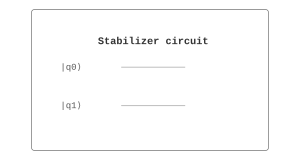
\includegraphics[width=0.6\textwidth]{../../images/stabilizer_circuit.svg}
\end{center}

\subsection{数学推导}

稳定子码：
\begin{equation}
S = \langle g_1, g_2, \ldots, g_{n-k} \rangle
\end{equation}

其中 $g_i$ 是稳定子生成元。

\textbf{编码空间}：
\begin{equation}
\mathcal{C} = \{|\psi\rangle : g_i|\psi\rangle = |\psi\rangle, \forall i\}
\end{equation}

\textbf{逻辑算子}：
\begin{equation}
\bar{X}_i, \bar{Z}_i \in N(S) \setminus S
\end{equation}

\subsection{几何解释}

稳定子形式在群空间中描述量子纠错码。稳定子生成元定义了编码空间，逻辑算子定义了逻辑操作。

\section{代码详解}

\begin{verbatim}
from quonic.qec import stabilizer

# stabilizer(generators)
# generators: 稳定子生成元列表

result = stabilizer(
    generators=['ZZI', 'IZZ', 'XII']
)

# result.distance: 码距
# result.logical_operators: 逻辑算子
# result.encoding: 编码电路
print(f'Code distance: {result.distance}')
print(f'Logical operators: {result.logical_operators}')
\end{verbatim}

\section{进阶用法}

\subsection{场景 1：不同稳定子码}

\begin{verbatim}
from quonic.qec import stabilizer

# 不同稳定子码
s1 = ['ZZI', 'IZZ', 'XII']  # Steane 码
s2 = ['ZZII', 'IZZI', 'IIZZ', 'XXXX']  # 表面码
s3 = ['ZZZ', 'ZIZ', 'IZZ']  # 比特翻转码

for s in [s1, s2, s3]:
    result = stabilizer(s)
    print(f'Distance: {result.distance}')
\end{verbatim}

\subsection{场景 2：解码}

\begin{verbatim}
from quonic.qec import stabilizer

# 解码
result = stabilizer(['ZZI', 'IZZ', 'XII'])
syndrome = result.decode(error='X', position=0)
print(f'Syndrome: {syndrome}')
\end{verbatim}

\subsection{场景 3：容错操作}

\begin{verbatim}
from quonic.qec import stabilizer

# 容错操作
result = stabilizer(['ZZI', 'IZZ', 'XII'])
circuit = result.fault_tolerant_circuit(operation='CNOT')
print(f'Circuit: {circuit}')
\end{verbatim}

\section{适用场景}

\subsection{量子纠错}

稳定子形式是量子纠错码的统一框架。许多量子纠错码（如 Steane 码、表面码）都是稳定子码。

\subsection{量子密钥分发}

稳定子形式可以用于量子密钥分发中的错误检测。稳定子测量可以检测窃听行为。

\subsection{量子计算}

稳定子形式可以用于容错量子计算。稳定子码可以保护量子信息免受噪声影响。

\section{常见问题}

\subsection{稳定子形式和量子纠错码有什么关系？}

稳定子形式是量子纠错码的统一框架。许多量子纠错码（如 Steane 码、表面码）都是稳定子码。

\subsection{稳定子码的码距如何计算？}

稳定子码的码距是 $N(S) \setminus S$ 中最小权重的元素。

\section{学习路径}

\subsection{前置知识}
\begin{itemize}
  \item 量子纠错码
  \item 群论
  \item Pauli 算子
\end{itemize}

\subsection{继续学习}
\begin{itemize}
  \item Steane 码
  \item 表面码
  \item 容错量子计算
\end{itemize}

\section{完整示例代码}

\subsection{示例 1：基本稳定子码}

\begin{verbatim}
from quonic.qec import stabilizer

result = stabilizer(['ZZI', 'IZZ', 'XII'])
print(f'Code distance: {result.distance}')
\end{verbatim}

\section{下载}

\begin{itemize}
  \item [stabilizer.py](https://github.com/ChrisLee0721/QuoNic/blob/main/examples/stabilizer/stabilizer.py)
\end{itemize}

\end{document}
